\section{Problemas adicionales de termodinámica}
\rfigure
%
\pma{
Una pared de ladrillo de $\SI{20}{\centi\metre}$ de espesor y conductividad térmica $\SI{5E-4}{cal/(\second.\centi\metre.\celsius)}$, separa una habitación en la que el aire tiene una temperatura de $\SI{15}{\celsius}$, del exterior que tiene una temperatura de $\SI{-5}{\celsius}$. Si el coeficiente de convección interior es de $\SI{1E-4}{cal/(\second.\centi\square\metre.\celsius)}$ y el doble de  éste en el exterior, calcular: \textit{a}) La temperatura de la superficie interior de la pared. \textit{b}) La temperatura de la superficie exterior de la pared.
\\ \rta{0.95}{\textit{a}) $\SI{11.4}{\celsius}$; \textit{b}) $\SI{-3.16}{\celsius}$}
}
%
\pma{\label{p:P901}
La figura \ref{f:P901} es un esquema de una pared formada por dos planchas paralelas de $\SI{5}{\centi\metre}$ y $\SI{4}{\centi\metre}$ de grosor separadas por una intercámara (de aire) y con coeficientes de conductividad térmica de $\SI{209}{\watt.\metre^{-1}.\kelvin^{-1}}$ y $\SI{83.6}{\watt.\metre^{-1}.\kelvin^{-1}}$ respectivamente. Siendo $\SI{100}{\celsius}$ y $\SI{10}{\celsius}$ las temperaturas de las caras opuestas respectivas, determine la temperatura de la intercámara.
\\ \rta{0.95}{$\SI{70}{\celsius}$}
}
%
\begin{figure}[ht!]
  \begin{center}
    \includegraphics[scale=1]{termodinamica/img/termo_transmision_intercamara.png}
    \caption{Problema \ref{p:P901}.}\label{f:P901}
  \end{center}
\end{figure}
%
\pma{\label{p:P902}
La figura \ref{f:P902} muestra un corte longitudinal de una pared compuesta por $\SI{15}{\centi\metre}$ de hormigón y $\SI{3}{\centi\metre}$ de un revestimiento. La superficie libre del revestimiento se encuentra en contacto con aire a una temperatura $T_1 = \SI{20}{\celsius}$ y la superficie libre del hormigón con aire a $T_2 = \SI{0}{\celsius}$. La conductividad térmica de este hormigón es $\SI{0.65}{kcal.\metre^{-1}.h^{-1}.\celsius^{-1}}$. Se sabe que la cantidad de calor que se transmite a través de esta
pared por unidad de tiempo y por unidad de área es $\SI{48}{kcal.h^{-1}.\metre^{-2}}$. \textit{a}) ¿Cuánto vale el coeficiente de conductividad térmica del revestimiento? \textit{b}) ¿Cuál es la temperatura en la superficie de contacto entre el revestimiento y el hormigón? \textit{c}) Resuelva nuevamente el problema pero ahora incluyendo convección a ambos lados de la pared. Considere que el coeficiente de convección del aire en el interior es $\SI{5}{\watt/(\square\metre.\kelvin)}$ y el del aire en el exterior es $\SI{12}{\watt/(\square\metre.\kelvin)}$.
\textit{d}) Realice un gráfico de la temperatura como función de la posición dentro de la pared.
\\ \rta{0.95}{\textit{a}) $\SI{0.162}{kcal.\metre^{-1}.h^{-1}.\celsius^{-1}}$; \textit{b}) $\SI{11.1}{\celsius}$; \textit{c})}
}
%
\begin{figure}[h!]
  \begin{center}
    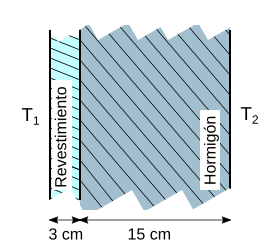
\includegraphics[scale=1]{termodinamica/img/termo_transmision_hormigon.png}
    \caption{Problema \ref{p:P902}.}\label{f:P902}
  \end{center}
\end{figure}
%
\pma{
Se coloca una cantidad de gas en un cilindro metálico que tiene un émbolo móvil en un extremo. No hay fugas de gas del cilindro a medida que el pistón se mueve. La fuerza externa aplicada al pistón se puede variar para cambiar la presión del gas a medida que se mueve el pistón para cambiar el volumen
del gas. Un manómetro unido a la pared interior del cilindro mide la presión del gas y se puede calcular el volumen del gas a partir de una medición de la posición del pistón en el cilindro. Se comienza con una presión de $\SI{1.0}{atm}$ y un volumen de gas de $\SI{3.0}{\liter}$. Manteniendo la  presión constante, se aumenta el volumen a $\SI{5.0}{\liter}$. Luego, manteniendo el volumen constante en $\SI{5.0}{\liter}$, se aumenta la presión a $\SI{3.0}{atm}$. A continuación, se disminuye la presión linealmente en función del volumen hasta que el volumen sea de $\SI{3.0}{\liter}$ y la presión sea de $\SI{2.0}{atm}$. Finalmente, se mantiene el volumen constante a $\SI{3.0}{\liter}$ y se disminuye la presión a $\SI{1.0}{atm}$, devolviendo el gas a su presión y volumen iniciales. Las paredes del cilindro son buenos conductores del calor, a través de las cuales se realizan los flujos de calor necesarios para estas transformaciones. A estas presiones relativamente altas, usted sospecha que la ecuación de gas ideal no se aplicará con mucha precisión. Usted no sabe qué gas está en el cilindro o si es monoatómico, diatómico o poliatómico. ¿Cuál es el calor neto para el gas durante este ciclo? ¿Hay flujo calor neto hacia adentro o hacia afuera del gas?
\\ \rta{0.95}{$Q = \SI{-304}{\joule}$. Hay un flujo neto de calor hacia afuera del gas}
}
%
\pma{
En cierto proceso, un sistema desprende $\SI{0.215}{\mega\joule}$ de calor, al tiempo que se contrae bajo una presión externa constante de $\SI{0.95}{\mega\pascal}$. La energía interna del sistema es la misma al principio y al final del proceso. Calcule el cambio de volumen del sistema.
\\ \rta{0.95}{$\Delta V = \SI{-0.226}{\cubic\metre}$}
}
%
\pma{
Una máquina de Carnot tiene una eficiencia del 59\% y realiza $\SI{25}{\kilo\joule}$ de trabajo en cada ciclo. \textit{a}) ¿Cuánto calor extrae la máquina de su fuente de calor en cada ciclo? \textit{b}) Suponga que la máquina expulsa calor a una temperatura ambiente de $\SI{20}{\celsius}$. ¿Cuál es la temperatura de su fuente de calor?
\\ \rta{0.95}{\textit{a}) $\SI{42.37}{\kilo\joule}$; \textit{b}) $\SI{442}{\celsius}$}
}
%
\pma{\label{p:P707}
Considere un ciclo Diesel idealizado como el que se muestra en la figura \ref{f:P707}, que inicia  (punto \textit{a}) con aire a una temperatura $T_a$. El aire puede tratarse como gas ideal. Calcule la eficiencia si $T_a = \SI{300}{\kelvin}$, $T_c = \SI{950}{\kelvin}$, $\gamma = 1.4$ y $r = 15$. AGREGAR PREGUNTA ESTILO COMO SE DEBE MODIFICAR PARA AUMENTAR SU RENDIMIENTO.
\\ \rta{0.95}{$0.657$}
}
\begin{center}
  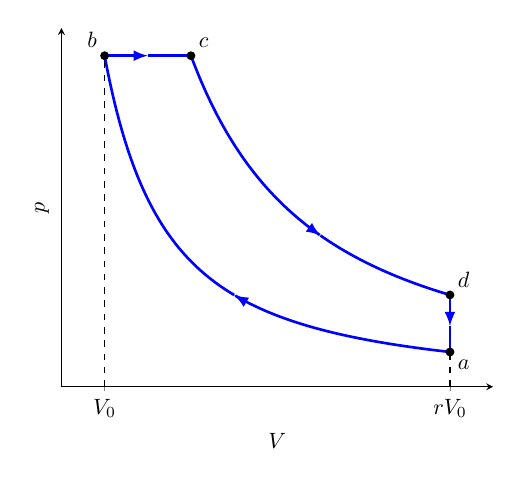
\begin{tikzpicture}[scale=0.8]
    \begin{axis}[
      % ticks=none,
      axis x line=bottom,
      axis y line=left,
      xmin=0.5, xmax=5.5,
      ymin=0, ymax=650,
      xlabel={$V$},
      ylabel={$p$},
      xtick={1,5},
      xticklabels={$V_0$,$rV_0$},
      ytick=\empty,
      % yticklabels={}
      %extra x ticks={0.04},
      %extra y ticks={2}
      ];
    \addplot [latex-, color=blue, very thick] [samples= 180, domain=2.5:5] {600/x^1.4};
    \addplot [color=blue, very thick] [samples= 180, domain=1:2.5] {600/x^1.4};
    \addplot [-latex, color=blue, very thick] [samples= 180, domain=2:3.5] {1583.41/x^1.4};
    \addplot [color=blue, very thick] [samples= 180, domain=3.5:5] {1583.41/x^1.4};

    \addplot[-latex, color = blue, very thick] coordinates {(1,600) (1.5, 600)};
    \addplot[color = blue, very thick] coordinates {(1.5,600) (2, 600)};
    \addplot[-latex, color = blue, very thick] coordinates {(5,166.355) (5,110)};
    \addplot[color = blue, very thick] coordinates {(5,110) (5, 63.04)};

    \addplot[color = black, dashed, thick] coordinates {(1, 0) (1, 600)};
    \addplot[color = black, dashed, thick] coordinates {(5, 0) (5, 63)};

    \draw (1,600) node [above left] {$b$};
    \draw (2,600) node [above right] {$c$};
    \draw (5,166.4) node [above right] {$d$};
    \draw (5,63) node [below right] {$a$};
    \fill [black](1,600) circle(2pt);
    \fill [black](2,600) circle(2pt);
    \fill [black](5,166.4) circle(2pt);
    \fill [black](5,63) circle(2pt);
    \end{axis}
  \end{tikzpicture}
  \captionof{figure}{Problema \ref{p:P707}\label{f:P707}}
\end{center}
%
% \begin{figure}[h!]
%     \begin{center}
%       \includegraphics[scale=0.75]{termo_2doppio_ciclo_diesel.png}
%       \caption{Problema \ref{p:P707}.}\label{f:P7007}
%     \end{center}
% \end{figure}
%
\pma{
{\color{red} ¿Eliminar?} Un recipiente rígido y perfectamente aislado tiene una membrana que divide su volumen en mitades. Un lado contiene un gas a una temperatura absoluta $T_0$ y presión $p_0$, mientras que la otra mitad está completamente vacía. De repente, se forma un pequeño orificio en la membrana, permitiendo que el gas se filtre hacia la otra mitad hasta que termina por ocupar el doble de su volumen original. En términos de $T_0$ y $p_0$, ¿cuál será la nueva temperatura y presión del gas cuando se distribuye equitativamente en ambas mitades del recipiente?
}
%
\pma{
Si se conocen los estados inicial y final de un sistema y el cambio correspondiente de energía interna, ¿podría determinarse si dicho cambio se debió a trabajo o a transferencia de calor?
}
%
\pma{
{\color{red} ¿Eliminar?} Usted sostiene un globo inflado sobre un conducto de aire caliente de su casa y observa que se expande lentamente. Después, usted lo aleja del conducto y lo deja enfriar a la temperatura ambiente. Durante la expansión, ¿cuál era mayor, el calor agregado al globo o el trabajo efectuado por el aire dentro de este? (Suponga que el aire es un gas ideal). Una vez que el globo  regresa a la temperatura ambiente, ¿cómo se compara el calor neto ganado o perdido por el aire dentro del globo con el trabajo neto efectuado sobre el aire circundante o con el trabajo realizado por este último?
}
%
\pma{
{\color{red} Agregar precisión a la pregunta.} Suponga que trata de enfriar su cocina dejando abierta la puerta del refrigerador. ¿Qué sucede? ¿Por
qué? ¿El resultado sería el mismo si se dejara abierta una hielera llena de hielo? Explique las diferencias, si las hay.
}
%
\pma{
Las máquinas térmicas reales, como el motor de gasolina de un auto, siempre tienen fricción entre sus piezas móviles, aunque los lubricantes la reducen al mínimo. ¿Una máquina térmica con piezas totalmente sin fricción sería 100\% eficiente? ¿La respuesta depende de si la máquina realiza un ciclo de Carnot o no?
}
%
\pma{
¿La Tierra y el Sol están en equilibrio térmico? ¿Hay cambios de entropía asociados a la transmisión de energía del Sol a la Tierra?
}
%
\pma{
¿Qué eficiencia tendría una máquina de Carnot que opera con $T_\text{caliente} = T_\text{fría}$? ¿Y si  $T_\text{fría} = \SI{0}{\kelvin}$ y $T_\text{caliente}$ fuera cualquier temperatura mayor que $\SI{0}{\kelvin}$? Interprete sus respuestas.
}
%